\chapter{Neural Network}\label{chap:nn}

Neural networks, a subset of machine learning, have shown exceptional
capabilities in understanding and predicting patterns within data. Their
strength lies in their ability to learn from complex and high-dimensional data,
which makes them invaluable for applications like time series analysis.

\section{Selection of Neural Network Architecture}

Considering the sequential nature of our data, the primary requirement was a
neural network architecture adept at handling sequential or temporal data. This
requirement led us to consider several models specially designed for this type
of data.

\subsection{Recurrent Neural Networks}

\glspl{rnn} are a class of neural networks that excel in handling sequential data,
owing to their unique ability to model temporal dynamics \cite{doi:10.1073/pnas.79.8.2554}.
The defining characteristic of \glspl{rnn} is their recurrent hidden state,
which effectively functions as a form of memory. This state is updated at each
time step of the sequence, incorporating information from the current input as
well as the previous hidden state. Thus, \glspl{rnn} can carry forward the
information throughout the sequence, which is crucial for many tasks, such
as language modelling or time series prediction.

However, despite their strengths, \glspl{rnn} have a significant drawback known
as the vanishing gradients problem \cite{gradients:1994}. During the training
of a neural network using backpropagation, the gradients often become
exponentially small as they are back-propagated through time, particularly over
long sequences. This causes the weights of the network to be updated very
slowly and can lead to the earlier layers of the network learning very slowly
or not at all. This in effect limits the \gls{rnn}'s ability to model long-term
dependencies in the data.

\subsubsection{Long Short-Term Memory Networks}

One of the most popular and effective solutions to the vanishing gradient
problem is the \gls{lstm}, introduced by Hochreiter and Schmidhuber
\cite{lstm:1997}. \gls{lstm}s introduce the concept of a cell state, a form of
long-term memory, and three types of gates (input, forget, and output) that
control the flow of information into, out of, and within the cell.

The cell state acts as a conveyor belt that runs parallel to the chain-like
structure of the \gls{rnn}, allowing information to be carried forward with
minimal transformations. The gates, each of which consists of a sigmoid neural
net layer and a pointwise multiplication operation, selectively control which
information is retained or discarded at each time step.

This design enables \glspl{lstm} to learn when to forget previous hidden states
and when to update hidden states with new information, thus effectively
combating the vanishing gradients problem and allowing them to capture
long-term dependencies in the data.

\subsubsection{Gated Recurrent Unit Networks}

Another variant of the \gls{rnn} that addresses the vanishing gradients problem
is the \gls{gru} \cite{gru:2014}. A \gls{gru} has a similar goal as an
\gls{lstm}, but with a different approach. It simplifies the architecture by
using two gates (update and reset) and by merging the hidden state and cell
state.

The update gate determines how much of the previous state to keep around, while
the reset gate is used to decide how much of the previous state to forget.
Despite their simpler architecture, \glspl{gru} have been found to perform on
par with \glspl{lstm} on a variety of tasks while being computationally more
efficient.

\begin{figure}[H]
    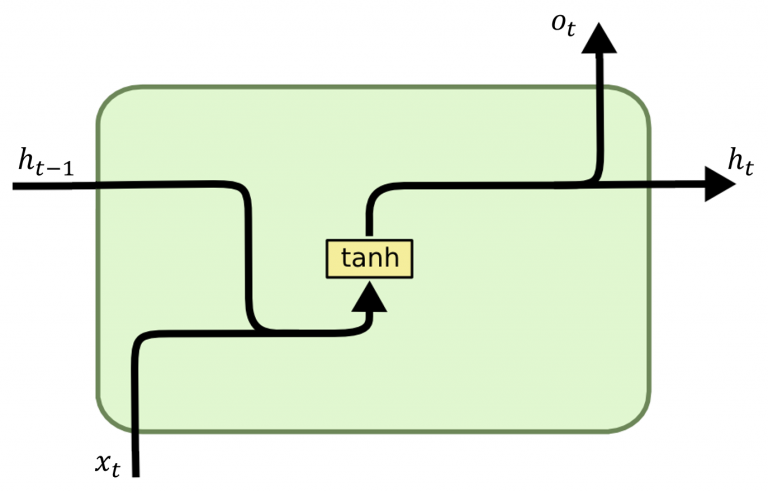
\includegraphics[width=0.3\textwidth]{files/RNN_Core2-768x491.png}
    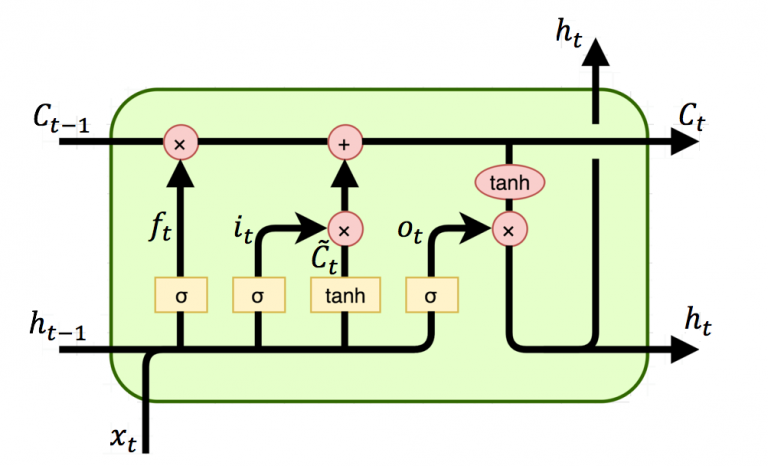
\includegraphics[width=0.3\textwidth]{files/LSTM-Core-768x466.png}
    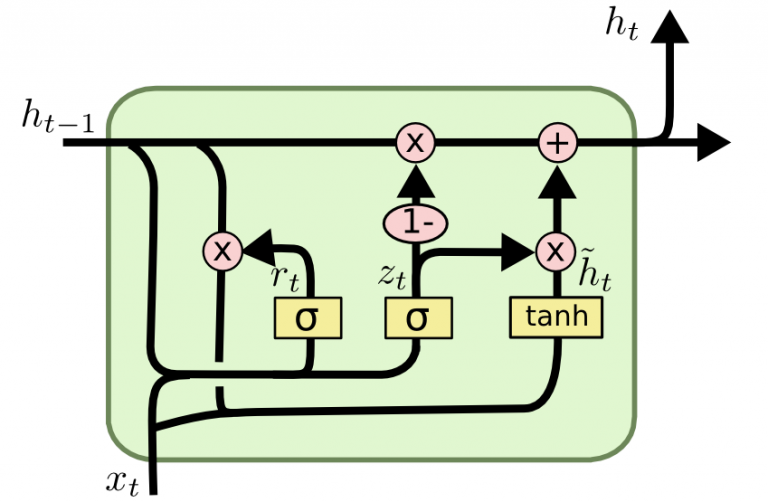
\includegraphics[width=0.3\textwidth]{files/GRU-768x502.png}
    \caption{Comparison of the core components of \gls{rnn}, \gls{lstm}, and \gls{gru} \cite{http://dprogrammer.org}}
\end{figure}

\subsection{Transformer Networks}

A more recent development in the neural network domain is Transformer networks
\cite{attention:2017}. These have achieved considerable success, particularly
in the field of natural language processing. Instead of relying on recurrence,
Transformer networks leverage an attention mechanism to weight the significance
of different portions of an input sequence, allowing them to focus on the most
relevant parts.

The key innovation of Transformer models is their focus on attention
mechanisms, particularly the so-called `Scaled Dot-Product Attention' and
`Multi-Head Attention'. In contrast to \glspl{rnn} which process sequence data
iteratively, attention mechanisms allow Transformers to process entire
sequences of data simultaneously, enabling them to capture long-range
dependencies in the data more effectively.

These are the key components of these networks networks:

\begin{itemize}
    \item \textbf{Scaled Dot-Product Attention:} This is the fundamental attention
          mechanism in Transformer models. Given a query, key, and value, it computes
          the dot product of the query with all keys, divides each by the square root
          of the key dimension, and applies a softmax function
          \footnote{The softmax function converts a vector of scalars into a
              vector of probabilities that are proportional to the relative scale
              of each value.} on the values.
          The output is the weighted sum of the values.

    \item \textbf{Multi-Head Attention:} This is simply a way of using multiple
          attention mechanisms (or `heads') in parallel, each with its learned linear
          transformations of the original queries, keys, and values. The outputs of
          each head are concatenated and linearly transformed to result in the final output.

    \item \textbf{Positional Encoding:} Since Transformers do not involve any
          recurrence or convolution operations, they lack any notion of the order of
          tokens in the sequence. To remedy this, positional encodings are added to
          the input embeddings, providing the model with explicit information about
          the relative or absolute position of the tokens in the sequence.
\end{itemize}

In addition to these components, Transformer networks utilize several fully
connected layers, layer normalization, and a significant amount of residual
connections, which help in training deep networks.

Transformers' effectiveness largely stems from their ability to focus on
different parts of the input sequence, which is particularly important when
understanding the context in complex sentences or documents. By assigning
different weights to different parts of the input, they can effectively capture
the dependencies between words or tokens regardless of their distance from each
other in the sequence.

Furthermore, Transformers' architecture enables parallel processing of
sequences, leading to significantly faster training times compared to recurrent
models like \glspl{rnn} or \glspl{lstm} However, they do tend to require more
memory and are often computationally intensive due to the attention mechanism's
complexity, particularly for long sequences.

Despite their success, Transformer networks have some limitations. They may not
capture the sequential nature of the data as effectively as \glspl{rnn}
\cite{rnntransformer:2022}. Furthermore, Transformer networks are inherently
more complex to implement and typically require larger datasets to fully
leverage their attention mechanism, a requirement we could not meet with our
current dataset size.

Taking these factors into account, we selected an architecture utilizing an
\gls{lstm}. This decision was influenced by \gls{lstm}'s ability to handle long
sequences and maintain essential information, mitigating the vanishing
gradients problem. Additionally, the implementation complexity and data
requirements were manageable within the scope of our project, making it a
balanced choice. We also tested using a \gls{gru}, but it did not perform as
well.

\section{Implementation of the Neural Network}

The custom LSTM-based neural network architecture we utilized for our study was
built using PyTorch~\cite{pytorch}. PyTorch is a popular, open-source machine
learning library, appreciated for its dynamic computational graph and memory
efficiency, which offers flexibility and speed during model development and
training.

\subsection{Patients with different number of sessions}

A vital feature of our dataset is the varying lengths of patient sessions,
which necessitates the need for accommodating sequences of different lengths.
PyTorch's \texttt{pack\_padded\_sequence} and \texttt{pad\_packed\_sequence}
functions are particularly useful in such scenarios. They allow efficient
packing and unpacking of sequences into a format known as
\href{https://pytorch.org/docs/stable/generated/torch.nn.utils.rnn.PackedSequence.html}{\texttt{PackedSequence}}.

A \texttt{PackedSequence} object is essentially a pair of two data structures:
\begin{itemize}
    \item A tensor that contains concatenated sequence data.
    \item A tensor of integers that represents the length of each sequence.
\end{itemize}

The purpose of packing a sequence is to allow maximum computational efficiency
while maintaining the ability to handle variable-length sequences. In essence,
a \texttt{PackedSequence} tensor stores the data in a packed format, where the
sequence data are concatenated along the time dimension based on their lengths
in descending order. This storage format enables fast and efficient \gls{gpu}
computations and is particularly suited for use with recurrent layers like the
\gls{lstm}.

The \texttt{pack\_padded\_sequence} function converts padded sequences (where
shorter sequences are padded with zeros to match the maximum length) into
\texttt{PackedSequence} format. Conversely, the \texttt{pad\_packed\_sequence}
function reverses this process, converting a \texttt{PackedSequence} back into
padded sequences.

An additional tensor of \textit{lengths} was used in our implementation to hold
the actual length of each sequence in a batch. This tensor informs the LSTM
layer about the length of the input sequences, which allows it to correctly
ignore padded values beyond the length of each sequence. This functionality is
essential for processing batches of sequences with varying lengths while
avoiding computation on padding tokens.

\begin{figure}
    \centering
    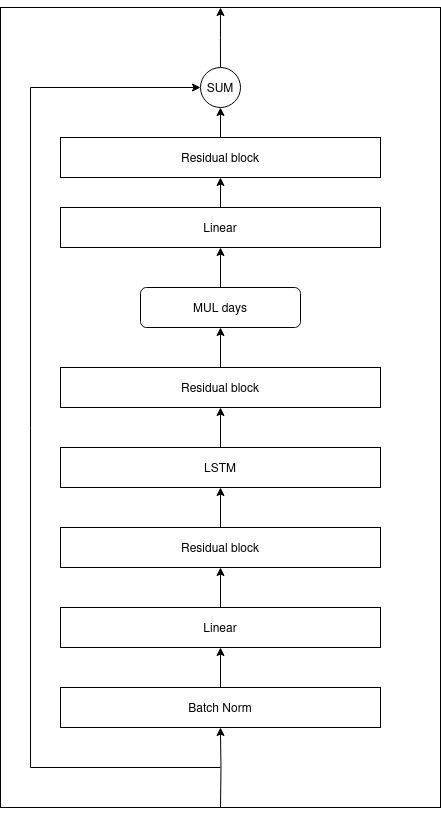
\includegraphics[width=8cm]{files/nn_diagram}
    \caption{Diagram of the implemented \gls{lstm}-based neural network architecture}
    \label{fig:nn_diagram}
\end{figure}

This approach accommodates our needs for dealing with variable-length sequences
and makes the most of PyTorch's efficient processing capabilities. It has been
central to the successful implementation of our LSTM-based neural network
architecture.

\subsection{Variability in the dates of the sessions}

The dataset's sessions are not uniformly spaced in time, varying from a few
days to several months apart. This is a problem for neural networks, since they
work best with uniformly spaced data. To solve this problem, we decided to make
the neural network predict the daily change instead.

This was accomplished by adding a residual connection between the input and the
output of the neural network, and multiplying the output by the number of days
until the next session. This way, the neural network can learn to predict the
daily change, and the output is scaled to the number of days until the next
session. Figure \ref{fig:nn_diagram} shows how this is implemented in a visual
way.

\subsection{Datasets and DataLoader}

PyTorch's Dataset and DataLoader classes are powerful abstractions that
simplify the task of data loading and preparation. They not only handle
batching of the data, but also allow for data shuffling and parallel
processing, which can be critical for leveraging the full potential of the
hardware at hand and training the model.

For our implementation, we created a custom Dataset and DataLoader class that
have the following features:

\begin{itemize}
    \item \textbf{Dataset:} This class extends the abstract Dataset class from PyTorch.
          It includes an initialization method that performs several preprocessing
          tasks on the provided data, such as filtering out clients with only one
          session, removing rows with missing values in the target columns, and
          mapping client IDs to indices. The overridden \texttt{\_\_getitem\_\_} method
          introduces a dropout mechanism to drop a fraction of the client's sessions.
          This may serve as a form of data augmentation. It then returns the processed
          data, which includes features, days between sessions, and target values.
          The \texttt{\_\_len\_\_} method returns the number of unique clients in the dataset.

    \item \textbf{DataLoader:} This class extends the DataLoader class from PyTorch.
          It uses a custom \texttt{collate\_fn} function to process the batches.
          The collate function takes a list of samples from the dataset and merges
          them into a single batch. Here, the collate function pads sequences to
          ensure that every sequence in a batch has the same length. It then calculates
          the lengths of each sequence and returns these along with the features,
          days between sessions, and target values. This class provides an iterable
          over the Dataset that ensures each batch is correctly processed and ready
          for training the model.
\end{itemize}

\section{Training and Optimization}

The neural network takes the following inputs:

\begin{itemize}
    \item A tensor of shape $(\text{batch size}, \text{max sequence length}, \text{number
                  of features})$.
    \item A tensor of shape $(\text{batch size}, 1)$ containing the length of the current
          sequence.
    \item A tensor of shape $(\text{batch size}, \text{max sequence length}, 1)$
          representing the number of days until the next session.
\end{itemize}

The neural network returns:

\begin{itemize}
    \item A tensor of shape $(\text{batch size}, \text{max sequence length}, \text{number
                  of features})$ that contains the predicted values for the next session for
          every session of every patient in the batch.
\end{itemize}

Having the neural network generate all future sessions at once allows us to
parallelize the training process, which reduces the training time.

The input features are constructed by concatenating the $\beta$ parameters of
the \gls{smpl} model with the patient's height, weight, age and a one-hot
vector encoding their gender. Attempts to include body fat percentage and
muscle mass percentage did not yield improved results and were excluded to
prevent overfitting.

\subsection{Loss function}

A loss function, also known as a cost function, is a mathematical function that
quantifies how well a machine learning model performs a specific task. For a
neural network, the loss function measures the difference between the predicted
output of the model and the actual target values (the `truth'). The goal during
the training process is to minimize this loss, thereby making the model's
predictions as close as possible to the true values.

There are different types of loss functions depending upon the task. For
regression problems, a common loss function is \gls{mse}, which calculates the
square of the difference between the predicted and actual values, then averages
these across all samples. For binary classification problems, Binary
Cross-Entropy (also known as log loss) is often used, which quantifies the
difference between the true class and predicted probability. For multi-class
classification problems, Categorical Cross-Entropy is frequently used.

\begin{figure}[H]
    \begin{subfigure}{\textwidth}
        \[ \text{MSE}(y, \hat{y}) = \frac{1}{n} \sum_{i=1}^{n}(y_i - \hat{y}_i)^2 \]
    \end{subfigure}

    \begin{subfigure}{\textwidth}
        \[ \text{BCE}(y, \hat{y}) = -\frac{1}{n} \sum_{i=1}^{n} [y_i \log(\hat{y}_i) + (1 - y_i) \log(1 - \hat{y}_i)] \]
    \end{subfigure}

    \begin{subfigure}{\textwidth}
        \[ \text{CCE}(y, \hat{y}) = -\frac{1}{n} \sum_{i=1}^{n} \sum_{j=1}^{m} y_{ij} \log(\hat{y}_{ij}) \]
    \end{subfigure}
    \caption{Common loss functions}
\end{figure}

\subsection{Optimizer}

An optimizer is an integral component of training a neural network. It is the
mechanism that updates the model's parameters, specifically the weights and
biases, in response to the feedback provided by the loss function. The goal of
the optimizer is to minimize the loss function, thereby improving the accuracy
of the model's predictions. Different optimizers approach this problem in
unique ways, and the choice of optimizer can significantly impact the speed and
quality of the model's learning.

\textbf{\gls{sgd}} is a straightforward yet powerful optimization
algorithm. It estimates the error gradient for the current state of the model
using a subset of the data (a batch), and then updates the model's parameters
in the opposite direction of the gradient. This process is repeated, with the
model incrementally moving towards the region of minimum error in the parameter
space. Despite its simplicity, \gls{sgd} can be slow and susceptible to getting stuck
in local minima for complex models and loss function landscapes.

\begin{figure}[H]
    \[ w := w - \eta\nabla Q_i(w) \]
    \caption{\gls{sgd} update rule}
\end{figure}

\textbf{\gls{rmsprop}} is an adaptive learning rate method
designed to address some of the shortcomings of \gls{sgd}. \gls{rmsprop} changes the
learning rate by dividing it by an exponentially decaying average of squared
gradients. This method helps to attenuate the updates for frequent and high
gradients, thus allowing the optimizer to converge faster and reducing the
likelihood of getting stuck in local minima.

\begin{figure}[H]
    \begin{align*}
        g & := \beta g + (1 - \beta) (\nabla Q_i(w))^2,            \\
        w & := w - \frac{\eta}{\sqrt{g + \epsilon}} \nabla Q_i(w).
    \end{align*}
    \caption{\gls{rmsprop} update rule}
\end{figure}

\textbf{\gls{adam}} combines the best properties of \gls{rmsprop} and
momentum to provide an optimization method that can handle sparse gradients and
noisy data. It calculates an exponential moving average of the gradient and the
squared gradient, and the parameters beta1 and beta2 control the decay rates of
these moving averages. The moving averages themselves are estimates of the
first moment (the mean) and the second raw moment (the uncentered variance) of
the gradients. This combination allows \gls{adam} to achieve fast convergence and
high accuracy.

\begin{figure}[H]
    \begin{align*}
        m       & := \beta_1 m + (1 - \beta_1) \nabla Q_i(w),            \\
        v       & := \beta_2 v + (1 - \beta_2) (\nabla Q_i(w))^2,        \\
        \hat{m} & := \frac{m}{1 - \beta_1^t},                            \\
        \hat{v} & := \frac{v}{1 - \beta_2^t},                            \\
        w       & := w - \frac{\eta \hat{m}}{\sqrt{\hat{v}} + \epsilon}.
    \end{align*}
    \caption{\gls{adam} update rule}
\end{figure}

\textbf{\gls{adamw}} is a modification of the \gls{adam} optimizer that decouples the weight decay
from the optimization steps. While the original \gls{adam} applies weight decay
before the optimization step, \gls{adamw} applies it directly to the weights after
the step, which is a more direct form of weight decay, closer to L2
regularization. This decoupling can lead to better training results,
particularly with larger models and small batch sizes, and has since become a
popular choice in the deep learning community.

\begin{figure}[H]
    \begin{align*}
        m       & := \beta_1 m + (1 - \beta_1) \nabla Q_i(w),                               \\
        v       & := \beta_2 v + (1 - \beta_2) (\nabla Q_i(w))^2,                           \\
        \hat{m} & := \frac{m}{1 - \beta_1^t},                                               \\
        \hat{v} & := \frac{v}{1 - \beta_2^t},                                               \\
        w       & := (1 - \lambda \eta) w - \frac{\eta \hat{m}}{\sqrt{\hat{v}} + \epsilon}.
    \end{align*}
    \caption{\gls{adamw} update rule}
\end{figure}

We utilized the \gls{adamw} optimizer with a variable learning rate and weight
decay, along with \gls{mse} loss as the objective function.

During training, we employed early stopping to prevent overfitting. We
monitored the validation loss and stopped training if it did not improve for 50
epochs. We then loaded the model with the lowest validation loss and used it
for inference.

We used a factor of 0.2 in the training / test split, which resulted in 80\% of
the data being used for training and 20\% for testing.

\subsection{Hyperparameter tuning}

We performed a grid search to find the optimal hyperparameters for our model.
The hyperparameters we tuned are shown in
Table~\ref{tab:final-hyperparameters}.

\begin{table}[h]
    \centering
    \begin{tabular}{l c c}
        \toprule
        \textbf{Hyperparameter}                  & \textbf{Value} \\
        \midrule
        Batch size                               & 32             \\
        Number of layers in the input            & 4              \\
        Number of layers in the \gls{lstm}       & 4              \\
        Number of layers in the output           & 4              \\
        Number of hidden units in the \gls{lstm} & 32             \\
        Weight decay                             & 0.001          \\
        \bottomrule
    \end{tabular}
    \caption{Final hyperparameters used for the neural network}
    \label{tab:final-hyperparameters}
\end{table}

\section{Results}

\begin{figure}[h]
    \centering
    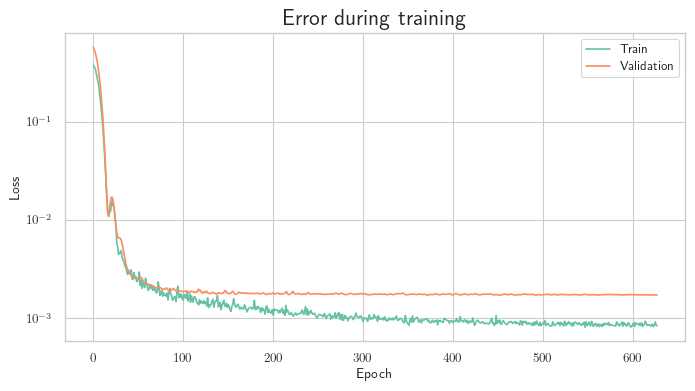
\includegraphics[width=\textwidth]{files/loss}
    \caption{MSE loss during training}
    \label{fig:loss}
\end{figure}

The training of the model was very sensitive to the set seed, which means that
the results varied significantly between runs. This is because the data is
split into training and validation sets at random, and there were only 15
patients assigned to the validation set. We decided not to change the seed
between runs, as we wanted to be able to compare the results of different
models.

We can see in Figure \ref{fig:loss} that the loss decreases rapidly in the
first few epochs, and then slowly converges to a minimum. The training loss
keeps decreasing, while the validation loss slows down but doesn't increase,
which indicates that the model is not overfitting.

\subsection{Predictions}

While a more detailed analysis of the results will be presented in the next
chapter, we provide some examples of our model's predictions.

Figure \ref{fig:predicted-betas} displays the shape parameters for a patient
alongside the model's prediction.

\begin{figure}[h]
    \centering
    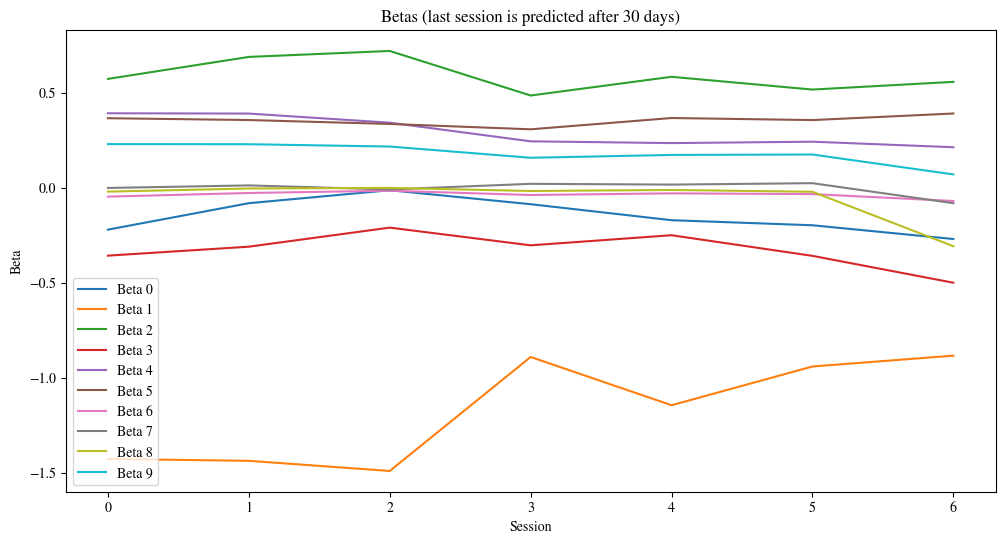
\includegraphics[width=\textwidth]{files/predicted_betas}
    \caption{Shape parameters for a patient and the model's prediction.}
    \label{fig:predicted-betas}
\end{figure}

Figure \ref{fig:patient-body-model} illustrates the reconstructed 3D model of a
patient's body, showcasing images from multiple sessions. The final image in
the sequence represents the model's prediction after one month from the last
session, with a total of 74 days between the first and last session.

\begin{figure}[h]
    \centering
    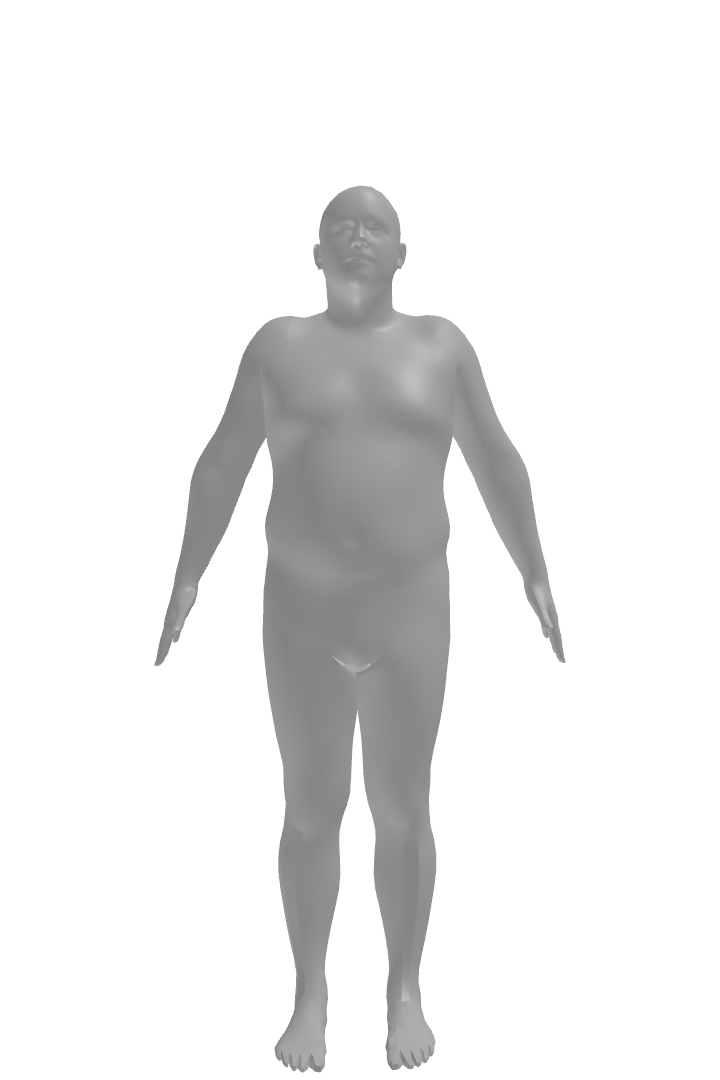
\includegraphics[width=120pt]{files/patients/2_6}
    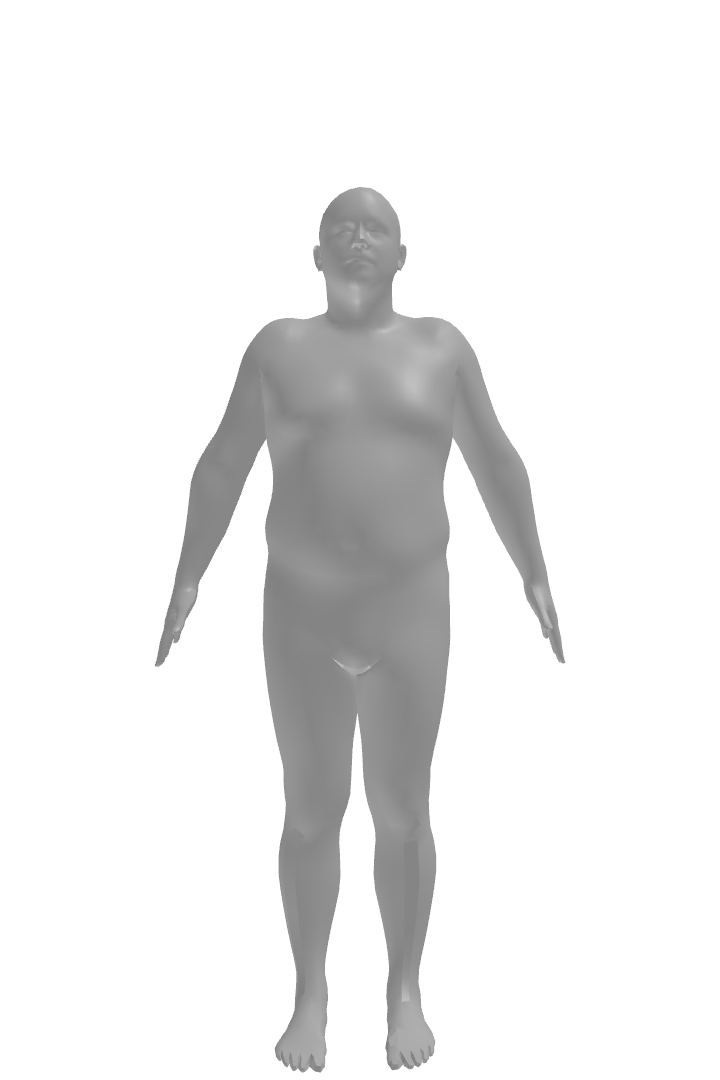
\includegraphics[width=120pt]{files/patients/2_7}
    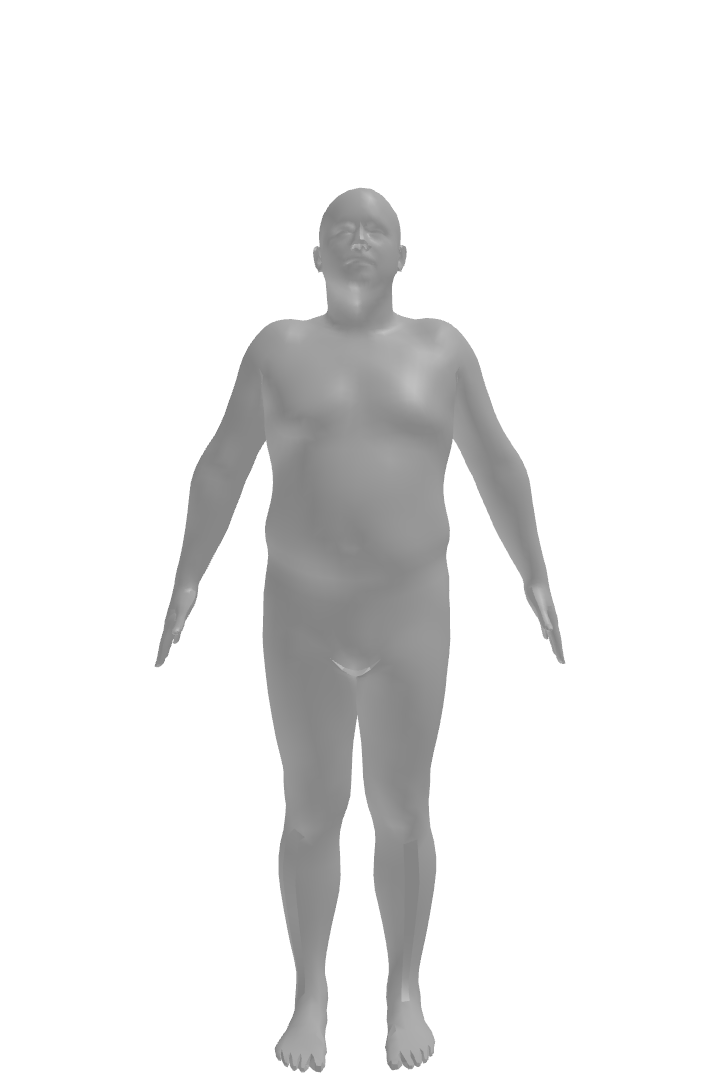
\includegraphics[width=120pt]{files/patients/2_8}
    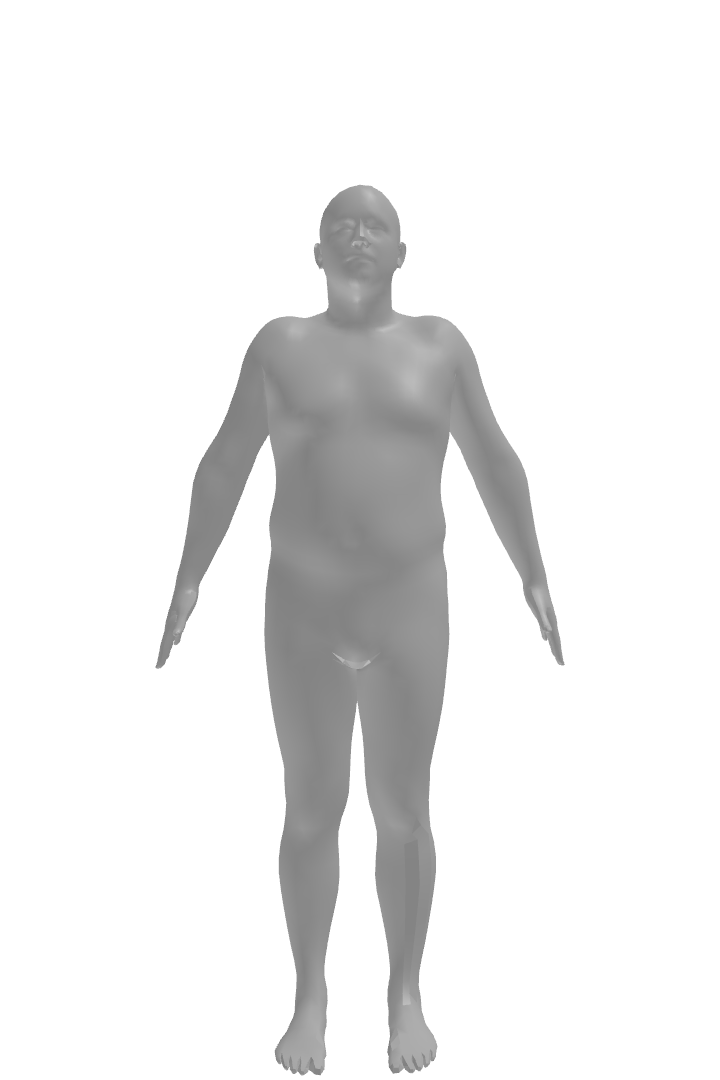
\includegraphics[width=120pt]{files/patients/2_9}
    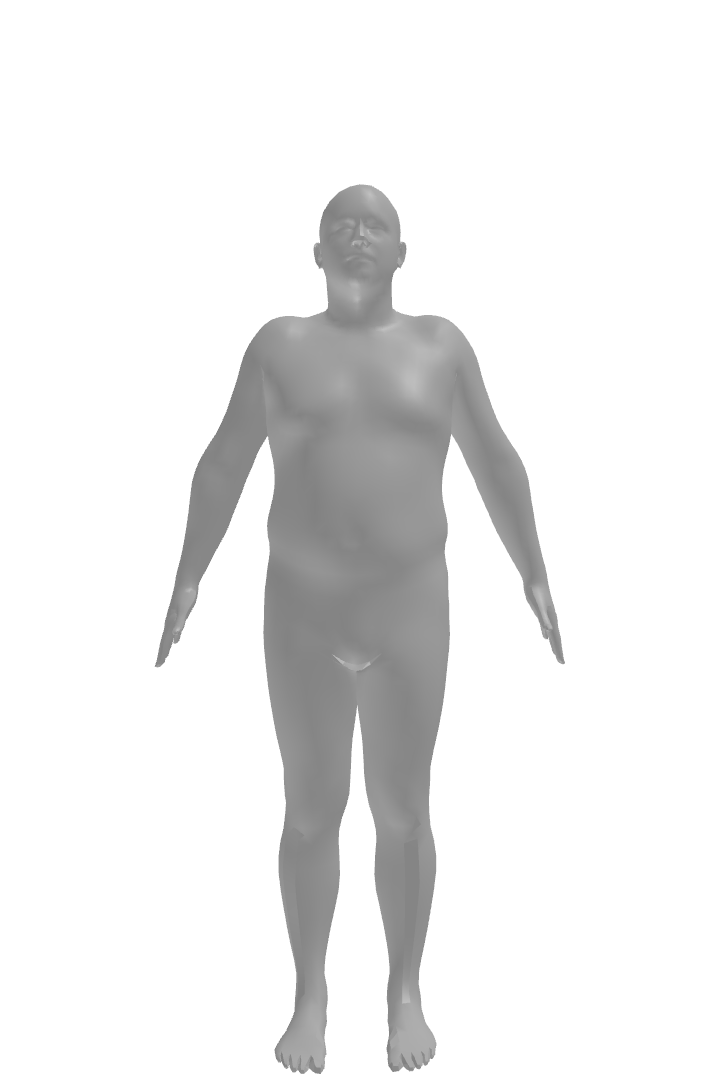
\includegraphics[width=120pt]{files/patients/2_10}
    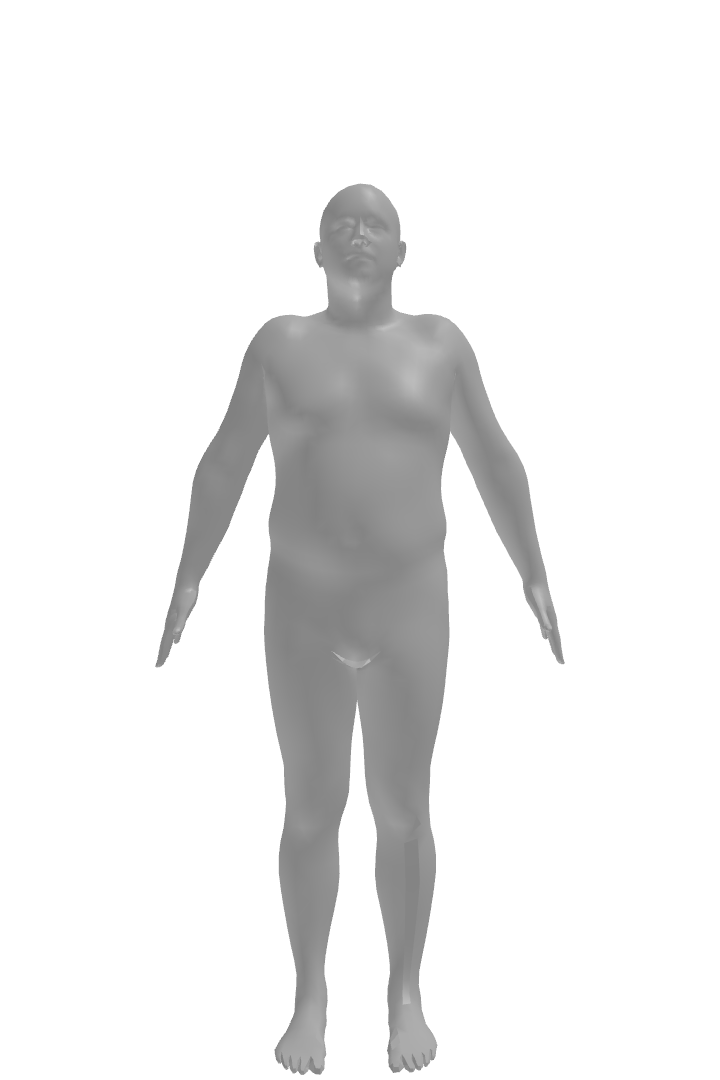
\includegraphics[width=120pt]{files/patients/2_11}
    \linebreak
    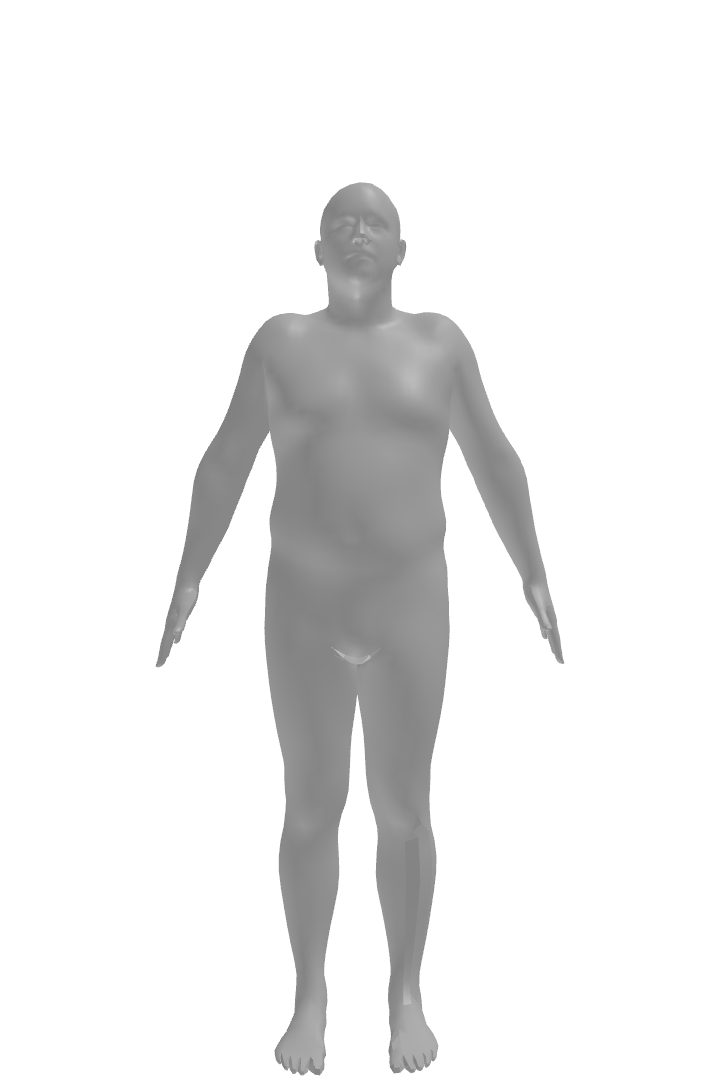
\includegraphics[width=120pt]{files/patients/2_predicted}
    \caption[Reconstructed 3D model of the patient's body]{Reconstructed 3D model of the patient's body. The last image is the model's prediction after one month from the last session. There are a total of 74 days between the first and last session.}
    \label{fig:patient-body-model}
\end{figure}

The results obtained provide an initial understanding of the model's
performance and will be further examined and discussed in the subsequent
chapter.